\documentclass[12pt]{scrartcl}

% Author: Galgon, 26.2.2015
% kleine Korrektur: Arndt, 09.11.2015

\usepackage{amsmath}
%\usepackage{hyperref}
\usepackage[utf8]{inputenc}
\usepackage{tikz}
\usetikzlibrary{decorations.markings}

\pagestyle{empty}

\setlength{\parindent}{0em}

\def\yx{y(x)}
\def\yxp{y(x+1)}
\def\tyx{\widetilde{y}(x)}
\def\tyxp{\widetilde{y}(x+1)}
\def\yxs{y^2(x)}
\def\yxps{y^2(x+1)}
\def\tyxs{\widetilde{y}^2(x)}
\def\tyxps{\widetilde{y}^2(x+1)}

\def\xy{x(y)}
\def\xym{x(y-1)}
\def\txy{\widetilde{x}(y)}
\def\txym{\widetilde{x}(y-1)}
\def\xys{x^2(y)}
\def\xyms{x^2(y-1)}
\def\txys{\widetilde{x}^2(y)}
\def\txyms{\widetilde{x}^2(y-1)}

\def\fba{\frac{b^2}{a^2}}
\def\fab{\frac{a^2}{b^2}}

\def\dx{d(x)}
\def\dxp{d(x+1)}

\def\dy{d(y)}
\def\dym{d(y+1)}

\def\fof{\frac{1}{4}}

\begin{document}

\begin{center}
  {\textbf{\Large First-Order Incremental Ellipses}\\[1ex](Analogously to Script)}\\ 
\end{center}
\medskip

\section*{Region 1}

\begin{center}
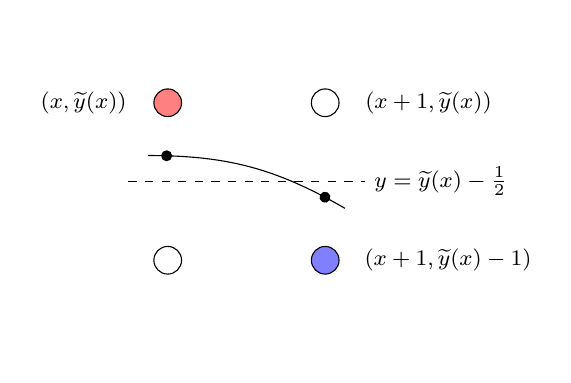
\begin{tikzpicture}
	\draw[draw=black,circle,fill=red!50!white] (0,2) circle (5pt) node[left=1em] {\footnotesize$(x,\tyx)$};
	\draw[draw=black,circle,fill=blue!50!white] (2,0) circle (5pt) node[right=1em] {\footnotesize$(x+1,\tyx-1)$};
	\draw[draw=black,circle,fill=white] (0,0) circle (5pt);
	\draw[draw=black,circle,fill=white] (2,2) circle (5pt) node[right=1em] {\footnotesize$(x+1,\tyx)$};
	\draw[black,decoration={
		markings,
		mark=at position 0.09 with {\fill circle (2pt);},
		mark=at position 0.89 with {\fill circle (2pt);}
	},postaction={decorate}] (-0.25,1.33) to[out=0,in=150] (2.25,0.66);
	\draw[black,dashed] (-0.5,1) -- (2.5,1) node[right] {\footnotesize$y=\tyx-\frac{1}{2}$};
\end{tikzpicture}
\end{center}

Decision for going south-east:

$$ \yxp < \tyx - \frac{1}{2} $$

$y$, $\widetilde{y}$ and $x$ all $\geq 0$, therefore

$$ \yxps < \tyxs - \tyx + \fof $$

Then, to not having to compute $\yxps$, with the ellipse formula

$$ \yxs = \frac{1}{a^2} \left( a^2b^2-b^2x^2 \right) = b^2 - \fba x^2 $$

we get

\begin{eqnarray*}
                                 b^2 - \fba (x+1)^2 &<& \tyxs - \tyx + \fof \\
\underbrace{b^2 - \fba x^2}_{\yxs} - 2\fba x - \fba &<& \tyxs - \tyx + \fof \\
                              \yxs - 2\fba x - \fba &<& \tyxs - \tyx + \fof
\end{eqnarray*}

And finally

\begin{equation} 
\dx := \yxs - \tyxs + \tyx - \fba(2x+1) - \fof < 0
\label{eq:dx}
\end{equation}

The decision $ \dx < 0 $ can be made without having to compute $\yxps$ 
but still requires $\yxs$. Now find an incremental update for $\dx$ to 
bypass computation of $\yxs$ in every step.

\subsubsection*{East}

$$ x \rightarrow x+1 \quad:\quad \tyxp = \tyx $$
\begin{align}
\dxp &= \yxps - \tyxps + \tyxp - \fba(2x+3) - \fof \nonumber \\
     &= \yxs - \fba(2x+1) - \tyxs + \tyx - \fba(2x+3) - \fof \nonumber \\
     &= \dx - \fba(2x+3)
\label{eq:dxe}
\end{align}

\subsubsection*{South-East}

$$ x \rightarrow x+1 \quad:\quad \tyxp = \tyx-1 $$
\begin{align}
\dxp &= \yxps - \tyxps + \tyxp - \fba(2x+3) - \fof \nonumber \\
     &= \yxs - \fba(2x+1) - (\tyx-1)^2 + \tyx - 1 - \fba(2x+3) - \fof \nonumber \\
     &= \yxs - \fba(2x+1) - \tyxs + 2\tyx - 1 + \tyx - 1 - \fba(2x+3) - \fof \nonumber \\
     &= \dx + 2\tyx - 2 - \fba(2x+3) \nonumber \\
     &= \dx + 2(\tyx - 1) - \fba(2x+3) \nonumber \\
     &= \dx + 2\tyxp - \fba(2x+3)
\label{eq:dxse}
\end{align}

\textbf{Note:} For an actual implementation it matters, whether the $y$
coordinate is decremented before or after the computation of $\dxp$.
This is reflected in the last step of the derivation. In this case, 
decrementing first, then computing $\dxp$ saves a few arithmetic 
operations (this is not really the case for $x$ here).

\subsubsection*{Kick-off}

In order to start this incremental scheme, $d(x_0)$ has to be 
initialized correctly. For an ellipse around $(0,0)$, the first point
on the ellipse is given as $(0,b)$. With Eq.(\ref{eq:dx}):

$$ d(x_0) = b^2 - b^2 + b - \fba - \fof = b - \fba - \fof $$

\textbf{Note:} As we are only interested in whether $\dx$ is larger or
smaller than $0$, the $\dx$ and their increments in Eqs.(\ref{eq:dxe}) 
and (\ref{eq:dxse}) can be scaled by constant factors, such as $a^2$
or $4$, ultimately allowing integer arithmetic everywhere.

\vspace*{1em}
\textbf{Note:} Region switch at $ a^2y = b^2x $. The question whether to
switch as soon as $\left( x+1, y-\frac{1}{2} \right)$ falls into region
$2$ or as soon as the first drawn point falls into region $2$ (or even
other conditions; one way might be to draw bottom-up) is kind of esoteric.

\section*{Region 2}

\begin{center}
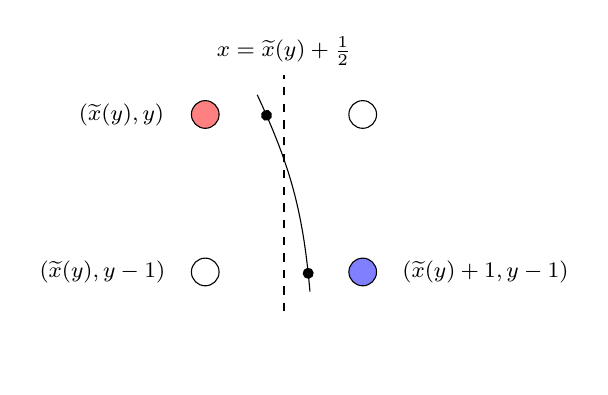
\begin{tikzpicture}
	\draw[draw=black,circle,fill=red!50!white] (0,2) circle (5pt) node[left=1em] {\footnotesize$(\txy,y)$};
	\draw[draw=black,circle,fill=blue!50!white] (2,0) circle (5pt) node[right=1em] {\footnotesize$(\txy+1,y-1)$};
	\draw[draw=black,circle,fill=white] (0,0) circle (5pt) node[left=1em] {\footnotesize$(\txy,y-1)$};
	\draw[draw=black,circle,fill=white] (2,2) circle (5pt);
	\draw[black,decoration={
		markings,
		mark=at position 0.09 with {\fill circle (2pt);},
		mark=at position 0.89 with {\fill circle (2pt);}
	},postaction={decorate}] (1.33,-0.25) to[out=95,in=-65] (0.66,2.25);
	\draw[black,dashed] (1,-0.5) -- (1,2.5) node[above] {\footnotesize$x=\txy+\frac{1}{2}$};
\end{tikzpicture}
\end{center}

Decision for going south:

$$ \xym < \txy + \frac{1}{2} $$

$x$, $\widetilde{x}$ and $y$ all $\geq 0$, therefore

$$ \xyms < \txys + \txy + \fof $$

Then, to not having to compute $\xyms$, with the ellipse formula

$$ \xys = \frac{1}{b^2} \left( a^2b^2-a^2y^2 \right) = a^2 - \fab y^2 $$

we get

\begin{eqnarray*}
                                 a^2 - \fab (y-1)^2 &<& \txys + \txy + \fof \\
\underbrace{a^2 - \fab y^2}_{\xys} + 2\fab y - \fab &<& \txys + \txy + \fof \\
                              \xys + 2\fab y - \fab &<& \txys + \txy + \fof
\end{eqnarray*}

And finally

\begin{equation} 
\dy := \xys - \txys - \txy + \fab(2y-1) - \fof < 0
\label{eq:dy}
\end{equation}

The decision $ \dy < 0 $ can be made without having to compute $\xyms$ 
but still requires $\xys$. Now find an incremental update for $\dy$ to 
bypass computation of $\xys$ in every step.

\subsubsection*{South-East}

$$ y \rightarrow y-1 \quad:\quad \txym = \txy+1 $$
\begin{align}
\dym &= \xyms - \txyms - \txym + \fab(2y-3) - \fof \nonumber \\
     &= \xys + \fab(2y-1) - (\txy+1)^2 - \txy - 1 + \fab(2y-3) - \fof \nonumber \\
     &= \xys + \fab(2x+1) - \txys - 2\txy - 1 - \txy - 1 + \fab(2y-3) - \fof \nonumber \\
     &= \dy - 2\txy - 2 + \fab(2y-3) \nonumber \\
     &= \dy - 2(\txy + 1) + \fab(2y-3) \nonumber \\
     &= \dy - 2\txym + \fab(2y-3)
\label{eq:dyse}
\end{align}

\textbf{Note:} For an actual implementation it matters, whether the $x$
coordinate is incremented before or after the computation of $\dym$.
This is reflected in the last step of the derivation. In this case, 
incrementing first, then computing $\dym$ saves a few arithmetic 
operations (this is not really the case for $y$ here).

\subsubsection*{South}

$$ y \rightarrow y-1 \quad:\quad \txym = \txy $$
\begin{align}
\dym &= \xyms - \txyms - \txym + \fab(2y-3) - \fof \nonumber \\
     &= \xys + \fab(2y-1) - \txys - \txy + \fab(2y-3) - \fof \nonumber \\
     &= \dy + \fab(2y-3)
\label{eq:dys}
\end{align}

\subsubsection*{Kick-off}

Let $(x_e,y_e)$ be the last computed point from region $1$. The 
initialization of $d(y_0)$ is then given, using Eq.(\ref{eq:dy}), as:

\begin{eqnarray*}
d(y_0) &=& x^2(y_e) - x_e^2 - x_e + \fab(2y_e-1) - \fof \\
       &=& a^2 - \fab y_e^2 - x_e^2 - x_e + \fab(2y_e-1) - \fof
\end{eqnarray*}

\textbf{Note:} Again we are only interested in whether $\dy$ is larger or
smaller than $0$. The $\dy$ and their increments in Eqs.(\ref{eq:dyse}) 
and (\ref{eq:dys}) can be scaled by constant factors, such as
$b^2$ or $4$, ultimately allowing integer arithmetic everywhere.

\end{document}
